% Section content template for individual Educative lessons
% This file contains the actual content for a specific section
% Generated from Educative API section content

% Section: Design of a Unique ID Generator
% Section ID: 5216880444309504
% Section Slug: design-of-a-unique-id-generator
% Generated: 2025-12-07T17:28:34.882947

In the \href{https://www.educative.io/courses/grokking-the-system-design-interview/system-design-sequencer}{previous} lesson, we saw how unique identifiers are used in many systems, for example, to label tweets, uploaded videos, or track execution flow across services. In this lesson, we will build on that by exploring different ways to design a system that generates such unique IDs. We will compare approaches like UUIDs, databases, and range handlers, and see how they meet key requirements identified in the following section.

\subsection{Requirements for unique identifiers}\label{EihVyTMdOtLr675uvt-lS}
\\
The requirements for our system are as follows:

\begin{itemize}
\item
\protect\phantomsection\label{GB3Ra0WLGouK7mfFjw_QE}
\textbf{Uniqueness}: We need to assign unique identifiers to different events for identification purposes.
\item
\protect\phantomsection\label{dUcm7cNpdboS81CR-I_EG}
\textbf{Scalability}: The ID generation system should generate at least a billion unique IDs per day.
\item
\protect\phantomsection\label{lVHsRGjBpSzGqEyfSMZSB}
\textbf{Availability}: Since multiple events happen even at the level of nanoseconds, our system should generate IDs for all the events that occur.
\item
\protect\phantomsection\label{jsviEe2sTT_5etJpd4F0s}
\textbf{64-bit numeric ID}: We restrict the length to 64 bits because this bit size is enough for many years in the future. Let's calculate the number of years after which our ID range will wrap around.
\end{itemize}

\[
\text{Total numbers available} = 2^{64} = 1.8446744 \times 10^{19}
\]

\[
\text{Estimated number of events per day} = 1 \ \text{billion} = 10^{9}
\]

\[
\text{Number of events per year} = 365 \ \text{billion} = 365 \times 10^{9}
\]

\[
\text{Number of years to deplete identifier range} = \frac{2^{64}}{365 \times 10^{9}} \approx 50{,}539{,}024.8595 \ \text{years}
\]

64 bits should be enough for a unique ID length, considering these calculations.
\\
Let's dive into the possible solutions for the problem mentioned above.

\subsection{First solution: UUID}\label{Tc5bkz2oqOMqIJjttIHMQ}
\\
A straw man solution(Often a simple solution whose primary purpose is to facilitate discussion towards better solutions.) for our design uses \textbf{UUIDs (universally unique IDs)}. This is a 128-bit number and it looks like \protect\phantomsection\label{katex_inline_tsaYIYNWiOi7LO8zz-SU4}{{{\(\text{123e4567e89b12d3a456426614174000}\)}}} in hexadecimal. It gives us about \protect\phantomsection\label{katex_inline_61PilKd9GTPlGPXq4UR-K}{{{\(10^{38}\)}}} numbers. UUIDs have different versions. We opt for version 4, which generates a pseudorandom number.
\\
Each server can generate its own ID and assign the ID to its respective event. No coordination is needed for UUID since it's independent of the server. Scaling up and down is easy with UUID, and this system is also highly available. Furthermore , it has a low probability of collisions. The design for this approach is given below:

\begin{figure}[htbp]
 \centering
 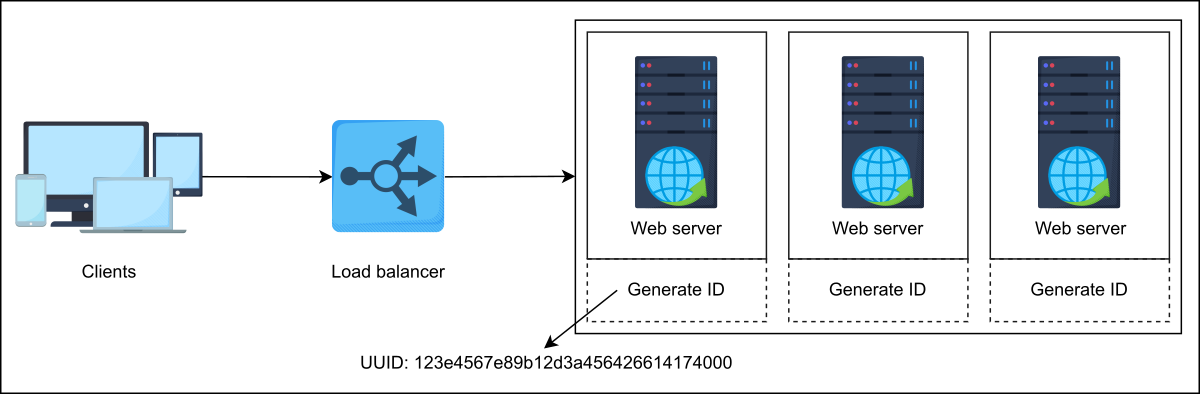
\includegraphics[width=0.5\textwidth]{Images/chapter_12/section_5216880444309504/6564473584615424.png}
 \caption{Generating a unique ID using the UUID approach}
\end{figure}

\subsection*{Point to Ponder}
\vspace{0.3cm}
\noindent
\textbf{Question 1:} What are the pros of using the UUID approach?
\\[0.2cm]
\begin{itemize}
 \item It doesn't require synchronization between servers.
 \item It's scalable.
 \item It's available.
 \item \textbf{[CORRECT]} All of the above
\end{itemize}

\subsubsection{Cons of using the UUID approach}\label{IuRDrxrEmG1AqX6rSNkPT}
\\
Using 128-bit numbers as primary keys makes the primary-key indexing slower, which results in slow inserts. A workaround might be to interpret an ID as a hex string instead of a number. However, non-numeric identifiers might not be suitable for many use cases. The ID isn't of 64-bit size. Moreover , there's a chance of duplication(UUID collision probability is low when there is sufficient randomness while implementing the UUID generator. 122 bits of UUID version 4 are set using a random or pseudo-random data source. If the randomness of such a data source is low, the collision probability can increase quite a bit.). Although this chance is minimal, we can't claim UUID to be deterministically unique. Additionally
, UUIDs given to clients over time might not be monotonically increasing. The following table summarizes the requirements we have fulfilled using UUID:

\textbf{Requirements Filled with UUID}

\begin{table}[htbp]
\centering
\small
\adjustbox{max width=\textwidth}{
\begin{tabular}{|p{0.236\textwidth}|p{0.170\textwidth}|p{0.156\textwidth}|p{0.138\textwidth}|p{0.250\textwidth}|}
\hline
\hfill\break & \textbf{Unique} & \textbf{Sca{} lable} & \textbf{Available} & \textbf{64-bit numeric ID} \\
\hline
\hline
\textbf{Using UUID} & no & yes & yes & no \\
\hline
\end{tabular}
}
\caption{Requirements Filled with UUID}
\end{table}

\subsection{Second solution: using a database}\label{D7PDYOdmo-XiG0E6qJfXy}
\\
Let's try mimicking the auto-increment feature of a database. Consider a central database that provides a current ID and then increments the value by one. We can use the current ID as a unique identifier for our events.

\begin{figure}[htbp]
 \centering
 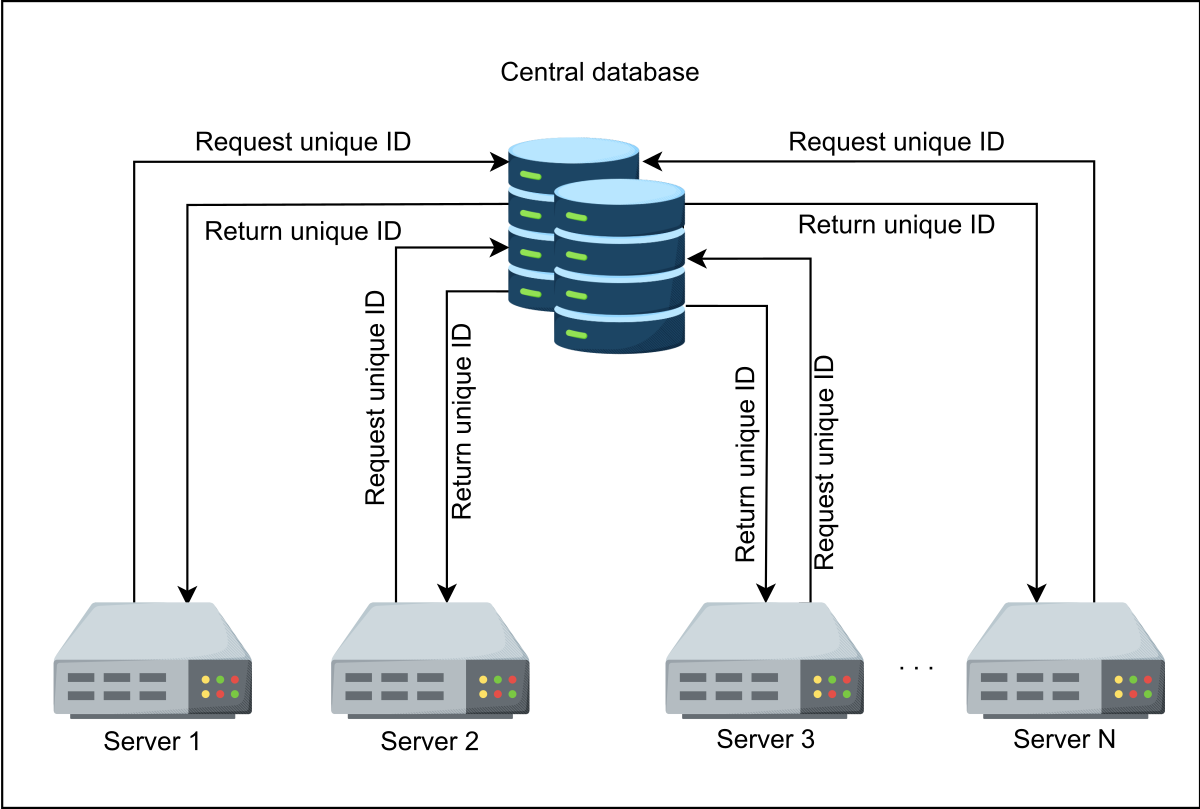
\includegraphics[width=0.5\textwidth]{Images/chapter_12/section_5216880444309504/5341708642811904.png}
 \caption{Using a central database to generate unique IDs}
\end{figure}

\begin{quote}
\textbf{Quiz:}
\textbf{Question 1:} What can be a potential problem of using a central database?
\textbf{Answer:} This design has a considerable problem: a single point of failure.

Reliance on one database can severely affect a system. The entire system will stop working if the central database goes down.
\end{quote}

To cater to the problem of a single point of failure, we modify the conventional auto-increment feature that increments by one. Instead of incrementing by one, let's rely on a value \texttt{m}, where \texttt{m} equals the number of database servers we have. Each server generates an ID, and the following ID adds \texttt{m} to the previous value. This method is scalable and prevents the duplication of IDs. The following image provides a visualization of how a unique ID is generated using a database:

\begin{figure}[htbp]
 \centering
 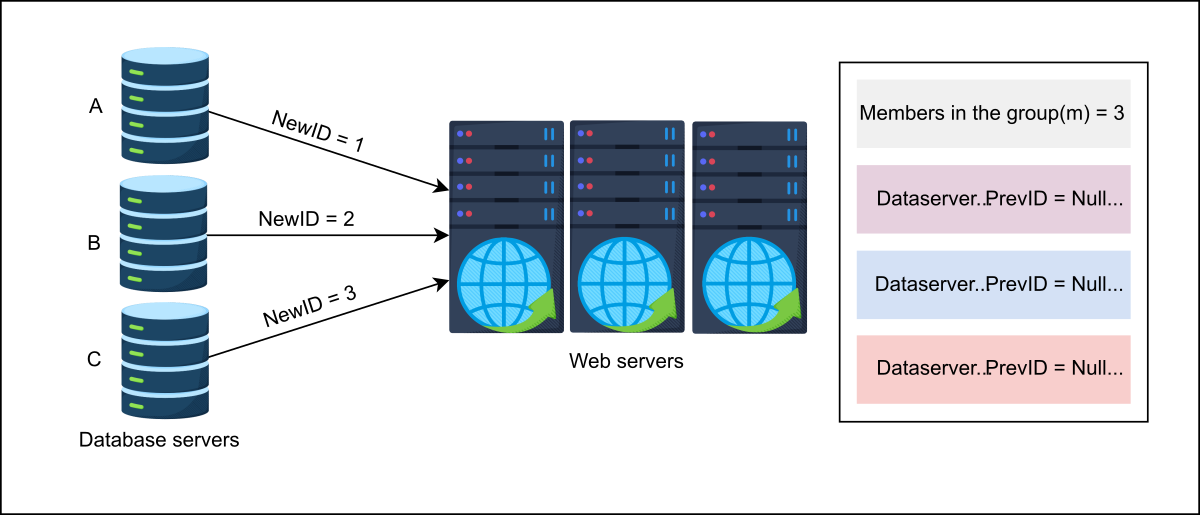
\includegraphics[width=0.5\textwidth]{Images/chapter_12/section_5216880444309504/5718337915322368.png}
 
\end{figure}

\subsubsection{Pros of using a database}\label{gkGGK8D9vMFPXphZE-_Xg}
\\
This approach is scalable. We can add more servers, and the value of \texttt{m} will be updated accordingly.

\subsubsection{Cons of using a database}\label{JkqW8vsjVfDsI3xMKnwY0}
\\
Though this method is somewhat scalable, it's difficult to scale for multiple data centers. The task of adding and removing a server can result in duplicate IDs. For example, suppose \texttt{m=3}, and server A generates the unique IDs 1, 4, and 7. Server B generates the IDs 2, 5, and 8, while server C generates the IDs 3, 6, and 9. Server
B faces downtime due to some failure. Now, the value \texttt{m} is updated to 2. Server A generates 9 as its following unique ID, but this ID has already been generated by server C. Therefore, the IDs aren't unique anymore.
\\
The table below highlights the limitations of our solution. A unique ID generation system shouldn't be a \textbf{single point of failure (SPOF)}. It should be scalable and available.

\textbf{Requirements Filled by UUID versus Using a Database}

\begin{table}[htbp]
\centering
\small
\adjustbox{max width=\textwidth}{
\begin{tabular}{|p{0.257\textwidth}|p{0.167\textwidth}|p{0.153\textwidth}|p{0.135\textwidth}|p{0.238\textwidth}|}
\hline
\hfill\break & \textbf{Unique} & \textbf{Scalable} & \textbf{Available} & \textbf{64-bit numeric ID} \\
\hline
\hline
\textbf{Using UUID} & no & yes & yes & no \\
\hline
\textbf{Using database servers} & no & yes & yes & yes \\
\hline
\end{tabular}
}
\caption{Requirements Filled by UUID versus Using a Database}
\end{table}

\subsection{Third solution: using a range handler}\label{iMi3LoN4xI7vQpNST0RAe}
\\
Let's try to overcome the problems identified in the previous methods. We can use ranges in a central server. Suppose we have multiple ranges for one to two billion, such as 1 to 1,000,000; 1,000,001 to 2,000,000; and so on. In such a case, a central microservice can provide a range to a server upon request.
\\
Any server can claim a range when it needs it for the first time or if it runs out of the range. Suppose a server has a range, and now it keeps the start of the range in a local variable. Whenever a request for an ID is made, it provides the local variable value to the requestor and increments the value by one.
\\
Let's say server 1 claims the number range 300,001 to 400,000. After this range claim, the user ID 300,001 is assigned to the first request. The server then returns 300,002 to the next user, incrementing its current position within the range. This continues until user ID 400,000 is released by the server. The application server then queries the central server for the next available range and repeats this process.
\\
This resolves the problem of the duplication of user IDs. Each application server can respond to requests concurrently. We can add a load balancer over a set of servers to mitigate the load of requests.
\\
We use a microservice called \textbf{range handler} that keeps a record of all the taken and available ranges. The status of each range can determine if a range is available or not. The state---that is, which server has what range assigned to it---can be saved on a replicated storage.
\\
This microservice can become a single point of failure, but a \textbf{failover server} acts as the savior in that case. The failover server hands out ranges when the main server is down. We can recover the state of available and unavailable ranges from the latest checkpoint of the replicated store.

\begin{figure}[htbp]
 \centering
 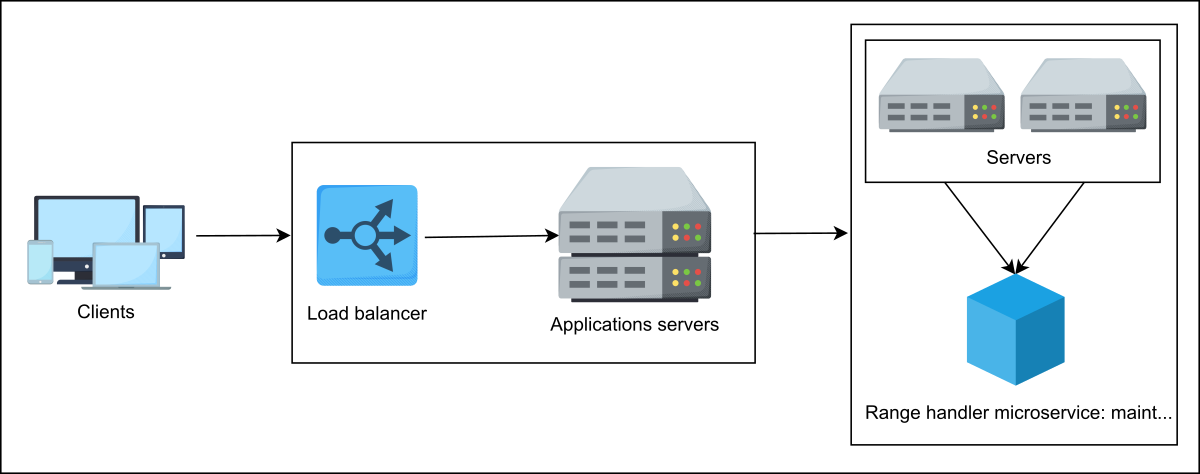
\includegraphics[width=0.5\textwidth]{Images/chapter_12/section_5216880444309504/5877090878881792.png}
 \caption{Design of the range handler microservice}
\end{figure}

Imagine a scenario where you're planning to bring a new data center online to accommodate increasing user requests. How would you modify your range allocation strategy to accommodate this change?

\textbf{Question:}

Adjusting range allocation for new data center

\textbf{Reference Answer:}

We can update our range allocation strategy to accommodate a new data center by distributing data ranges more evenly across all available data centers. One approach is to use geographic sharding, assigning data ranges based on user location to reduce latency. We can split existing ranges or migrate some ranges to the new location as we bring the new data center online. Consistent hashing can be applied to maintain balance and minimize disruption, allowing smooth range reallocation without major reshuffling. Additionally , implementing load balancing ensures that user requests are efficiently distributed across the infrastructure.

\subsubsection{Pros of using a range handler}\label{MDdI4JMCsaF9Ne0XCiIUS}
\\
This system is scalable, available, and yields user IDs that have no duplicates. Moreover, we can maintain this range in 64 bits, which is numeric.

\subsubsection{Cons of using a range handler}\label{bq9BHYztr92hCEjyjLuRI}
\\
We lose a significant range when a server dies and can only provide a new range once it's live again. We can overcome this shortcoming by allocating shorter ranges to the servers, although ranges should be large enough to serve identifiers for a while.
\\
The following table sums up what this approach fulfills for us:

\textbf{Requirements Filled by These Three Options}

\begin{table}[htbp]
\centering
\small
\adjustbox{max width=\textwidth}{
\begin{tabular}{|p{0.294\textwidth}|p{0.157\textwidth}|p{0.145\textwidth}|p{0.127\textwidth}|p{0.226\textwidth}|}
\hline
\hfill\break & \textbf{Unique} & \textbf{Sca{} lable} & \textbf{Available} & \textbf{64-bit numeric ID} \\
\hline
\hline
\textbf{Using UUID} & no & yes & yes & no \\
\hline
\textbf{Using database servers} & no & yes & yes & yes \\
\hline
\textbf{Using a range handler} & yes & yes & yes & yes \\
\hline
\end{tabular}
}
\caption{Requirements Filled by These Three Options}
\end{table}

We developed a solution that provides us with a unique ID, which we can assign to various events and even use as a primary key. But what if we add a requirement that the ID is time sortable too?

% End of section content